\documentclass[12pt, a4paper]{amsart}
\usepackage{amssymb}
\usepackage{amsthm}
\usepackage{amsfonts}
\usepackage{url}
\usepackage{tikz}
\usetikzlibrary{calc}
\newtheorem{lemma}{\bf Lemma}[section]
\newtheorem{proposition}[lemma]{\bf Proposition}
\newtheorem{observation}[lemma]{\bf Observation}
\parindent = 0mm
\parskip = 2mm
\begin{document}
\title{Two new approaches to string delimitations}
\author{Dominic van der Zypen}
%\address{Swiss Armed Forces, CH-3003 Bern, Switzerland}
%\email{dominic.zypen@gmail.com}
%\begin{abstract}
%\end{abstract}
%----------------------
\maketitle
%----------------------
\vspace*{-8mm}
\section{Problem setting}
Where does a string end? This is addressed using three different methods:
\begin{enumerate}
\item Number of characters in front of string: \\ {\tt 12:hello world!}
\item Quoting, and escaping quotes within string:\\ {\tt "hello,
\textbackslash "world\textbackslash ""}.
\item Delimiter such as EOF. Leads to problems when that
delimiter appears
in original string.
\end{enumerate}
This note used a modified version of (3) by constructing
for every string an {\em individual} delimiter $d(s)$
that does not appear in $s$. Then we can represent $s$ as
$$d(s):s:d(s)$$
So, for instance, if $s =$ {\tt hello world} we might have $d(s) =$ {\tt !}
and the representation of $s$ will be
\begin{quote}
{\tt !:hello world:!}
\end{quote}
In the following we discuss some ways of constructing $d(s)$ with these
goals in mind:
\begin{enumerate}
\item $d(s)$ must not be a substring of $s$,
\item $d(s)$ should be built in $O(n)$ time, where $n$ is the
length of the input string, and
\item the length of $d(s)$ should be kept as small as possible.
\end{enumerate}
%----------------------
\section{Two approaches}
\subsection{A simple counting algorithm} \label{counting}
Fix a character such as {\tt 7}
and assign to any string $s$ the non-negative integer $M(s)$ which
is defined in the following way:
\begin{quote}
Let $M(s)$ be the smallest number $k$ of consecutive instances
of {\tt 7} such that
$$\underbrace{\mathtt{77\ldots7}}_{k\text{ times}}$$
does {\bf not} appear in $s$.
\end{quote}
Then we let $d(s) = \underbrace{\mathtt{77 \ldots 7}}_{M(s)\text{ times}}$.

{\em Example.} Let $s = $ {\tt hello 7 world 77}. Then $M(s) =3$, since
$3$ is the smallest number $n$ such that {\tt 7} does not appear
$n$ consecutive times in the string $s$. So, $d(s) = $ {\tt 777}, and
the representation of $s$ is

\begin{quote}
{\tt 777:hello 7 world 77:777}
\end{quote}

It is easy to find a linear-time counting algorithm to determine $M(s)$
stepping through $s$ once.

The {\em disadvantage} of this representation is that $d(s)$ can
grow linearly with respect to $s$ in the worst case.
The next method we present will guarantee a length of the delimiter
of $O(\log(n))$ where $n$ is the length of the string. Also, we will
show that this is the best worst-case length you can get.
% - - - - - - - -
\subsection{Constant length moving window}\label{bit}
The overall goal of this paragraph will be to construct a
delimiter consisting of the characters {\tt 0} and {\tt 1}
such that
\begin{enumerate}
\item the length of the delimiter is $O(\log(n))$ where
$n$ is the length of the input string, and
\item finding the delimiter happens in $O(n)$ time.
\end{enumerate}
First, we will observe that it is not possible
to ``go below $O(\log(n))$ length''.

\begin{observation} Consider the following {\tt 0,1}-string of length 8: 
$$s = \mathtt{01110000}$$
We cannot
find a {\tt 0,1}-delimiter of length 2, as all of the {\tt 0,1}-strings
of length 2 (i.e., {\tt 00, 01, 10, 11}) appear in $s$. 
\end{observation}

Next we prove that $k = \lceil \log(n)\rceil+1$ is a sufficient 
substring length.

\begin{proposition} If $s$ is a {\tt 0,1}-string of length $n$ 
and $k := \lceil \log(n)\rceil+1$ there is 
 a {\tt 0,1}-string of length $k$ that is {\em not} a substring of $s$.
\end{proposition}
{\em Proof.} There are $n - k$ substrings in $s$ 
of length $k$, and there are $2^k$ {\tt 0,1}-strings of length $k$ 
in total. Since $n-k \leq 2^k - k < 2^k$, there must be a 
{\tt 0,1}-string of length $k$ that is not a $k$-length-substring of 
$s$. $\Box$

So we are armed to give a solution assuming that $s$ consists of characters
{\tt 0} and {\tt 1} only, and then show how we can reduce general strings
to {\tt 0,1}-strings.

\subsubsection{Solution for {\tt 0,1}-strings}\label{bit01}
Let $s$ be a given string consisting of characters {\tt 0} and {\tt 1} only.
Let $n \in \mathbb{N}$ be the length of $s$
and let $k := \lceil \log(n)\rceil+1$. Note that by $\log(\cdot)$ we
denote the logarithm of base $2$, and for any $x\in
\mathbb{R}$ we define
$$\lceil x \rceil = \inf\{z\in \mathbb{Z}: z\geq x\}.$$

We proceed along the following steps:
\begin{enumerate}
\item Initialise a {\em bit-field} $B$ of
length $2^k$ with constant value $0$.
\item Use a $k$-window to step through $s$  from beginning to end,
as depicted below:

\begin{center}
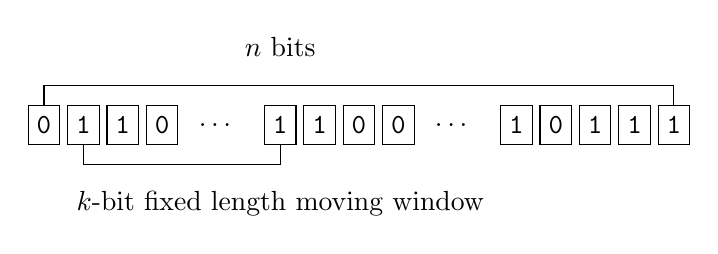
\begin{tikzpicture}[
   box/.style={rectangle,draw,minimum width=0.4cm,
    minimum height=0.5cm,inner sep=+0.1cm}
    ]
  % -- box row
  \node[box] at (1,0) (b12) {\tt 0};
  \node[box] at (1.5,0) (b11) { \tt 1};
  \node[box] at (2,0) (b10) {\tt 1};
  \node[box] at (2.5,0) (b9) {\tt 0};
  \node at (3.2,0) (b8) {\ldots};
  \node[box] at (4,0) (b6) {\tt 1};
  \node[box] at (4.5,0) (b5) {\tt 1};
  \node[box] at (5,0) (b4) {\tt 0};
  \node[box] at (5.5,0) (b3) {\tt 0};
  \node at (6.2,0) (b2) {\ldots};
  \node[box] at (7,0) (b0) {\tt 1};
  \node[box] at (7.5,0) (bm1) {\tt 0};
  \node[box] at (8,0) (bm2) {\tt 1};
  \node[box] at (8.5,0) (bm3) {\tt 1};
  \node[box] at (9,0) (bm4) {\tt 1};

  % -- brackets
    \draw[-] (bm4) -- ($(bm4) + (0,0.5)$) -- ($(b12) + (0,0.5)$) -- (b12);
    \draw[-] (b11) -- ($(b11) + (0,-0.5)$) -- ($(b6) + (0,-0.5)$) -- (b6);

  % -- labels
    \node at (4,1) {$n$ bits};
    \node at (4,-1) {$k$-bit fixed length moving window};

\end{tikzpicture}
\end{center}
\begin{center}
{\sc Figure 1.} The $k$-bit window moves through the string, and it is
interpreted as a $k$-bit binary number.
\end{center}

\vspace*{2mm}

\item For every $k$-substring, interpret the string as integer $x$
with $0 \leq x \leq 2^k - 1$ and in bit-field $B$, 
set bit number $x$ to $1$. Actually, this binary number will be 
stored in a {\tt uint64} variable {\tt w}, and the window rolling procedure 
can be quickly done in {\tt w}, see Appendix.
\item When this is completed, look for first bit-position set to $0$.
This gives a {\tt 0,1}-string not contained in original string!

\end{enumerate}
\subsubsection{Reducing general strings to {\tt 0,1}-strings}
This is the old parity trick: Step through every character (bit) of 
the given string $s$ and for every bit {\tt b} only save its parity
using bit-wise AND ({\tt \&}):
\begin{quote}
{\tt b = b \& 1;  // get 0 or 1 as bit}
\end{quote}
So we get a {\tt 0,1}-string $s_{0,1}$ out of $s$, and we proceed as above.
It is easy to see that the delimiter $d(s_{0,1})$ that the algorithm 
of \ref{bit01} produces does not appear in $s$.
\end{document}
